%=======INSTRUCTIONS FOR SIGNIFICANCE==========

\section*{A. Significance}

\begin{description} % For subheadings within a section, this template uses the {description} environment, it is not obtrusively large like a \subsection; and facilitates a brief optional subtitle; and it will wrap around figures and tables; it also has a decent amount of whitespace above/below which is less than for a section heading
\item[A.1. Instructions.]{Optional subtitle}
\end{description}

Explain the importance of the problem or critical barrier to progress in the field that the proposed project addresses.

Explain how the proposed project will improve scientific knowledge, technical capability, and/or clinical practice in one or more broad fields.

Describe how the concepts, methods, technologies, treatments, services, or preventative interventions that drive this field will be changed if the proposed aims are achieved.

\begin{description}
\item[A.2. Subheading.]{}
\end{description}

\begin{wraptable}{r}{4.8cm} % Example table with text wrapping around it
\caption{Example Table}
\begin{center}
\begin{tabular}{l l r}
\toprule
\multicolumn{1}{c}{City} & {N\textsuperscript{a}} & {\%Silly}\\
\midrule
San Diego & 289 & 41\%\\
Seattle & 262 & 32\%\\
Galveston & 261 & 15\%\\
St Louis & 269 & 7\%\\
New York & 271 & 4\%\\
Baltimore & 231 & 2\%\\
\emph{Total} & 1,586 & 21\%\\
\hline
\end{tabular}\\
\footnotesize\textsuperscript{a}{All participants clowns.}
\end{center}
\label{default}
\end{wraptable}

\lipsum[8-10]

\begin{wrapfigure}{r}{6.8cm} % Example figure with text wrapping around it
\includegraphics[scale=0.9]{Figures/Fig1.pdf}
\caption{\footnotesize Example wrapped figure. (A) Impressive microscopy image. (B) Impressive data.}
\end{wrapfigure}

\lipsum[5]

\begin{description}
\item[A.3. Another subheading:]{optional subtitle.}
\end{description}

\lipsum[25]

\begin{figure}[b] % Centered big figure at bottom of the page ([b] argument, could be "t" for top or "h" for here)
\centering
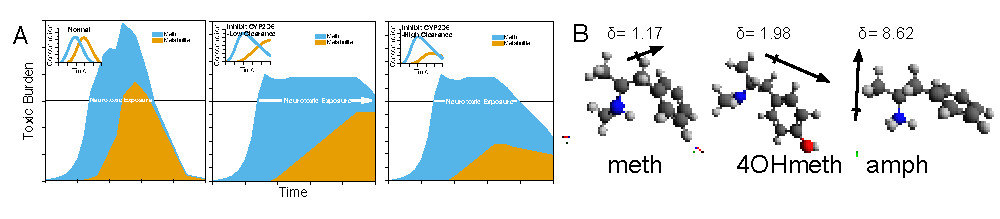
\includegraphics[scale = .80]{Figures/Fig2.pdf}
\caption{\footnotesize Big Figure legend Big Figure legend Big Figure legend Big Figure legend Big Figure legend Big Figure legend Big Figure legend Big Figure legend Big Figure legend.}
\label{fig2}
\end{figure}

\lipsum[31-32]

\begin{description}
\item[A.4. Yet another subheading.]{}
\end{description}

\lipsum[55-56]

%========INSTRUCTIONS FOR INNOVATION================

\section*{B. Innovation}

\begin{description}
\item[B.1. Instructions.]{}
\end{description}

Explain how the application challenges and seeks to shift current research or clinical practice paradigms.

Describe any novel theoretical concepts, approaches or methodologies, instrumentation or interventions to be developed or used, and any advantage over existing methodologies, instrumentation, or interventions.

Explain any refinements, improvements, or new applications of theoretical concepts, approaches or methodologies, instrumentation, or interventions.

%========INSTRUCTIONS FOR APPROACH================

\section*{C. Approach}

\begin{description}
\item[C.1. Instructions.]{}
\end{description}

Describe the overall strategy, methodology, and analyses to be used to accomplish the specific aims of the project. Unless addressed separately in Item 15 (Resource Sharing Plan), include how the data will be collected, analyzed, and interpreted as well as any resource sharing plans as appropriate.

Discuss potential problems, alternative strategies, and benchmarks for success anticipated to achieve the aims.

If the project is in the early stages of development, describe any strategy to establish feasibility, and address the management of any high risk aspects of the proposed work.

Point out any procedures, situations, or materials that may be hazardous to personnel and precautions to be exercised. A full discussion on the use of Select Agents should appear in Item 11, below.

As applicable, also include the following information as part of the Research Strategy, keeping within the three sections listed above: Significance, Innovation, and Approach.

\begin{description}
\item[C.2. Preliminary Studies for New Applications]{}
\end{description}

Preliminary Studies for New Applications: For new applications, include information on Preliminary Studies. Discuss the PD/PI's preliminary studies, data, and or experience pertinent to this application. Except for Exploratory/Developmental Grants (R21/R33), Small Research Grants (R03), and Academic Research Enhancement Award (AREA) Grants (R15), preliminary data can be an essential part of a research grant application and help to establish the likelihood of success of the proposed project. Early Stage Investigators should include preliminary data (however, for R01 applications, reviewers will be instructed to place less emphasis on the preliminary data in application from Early Stage Investigators than on the preliminary data in applications from more established investigators).

%------------------------------------------------
